\documentclass{beamer}

\usepackage[T1]{fontenc} 
\usepackage[latin1]{inputenc}
%% \usepackage[frenchb]{babel}

\usetheme{Warsaw}

% Supprimer les icones de navigation (pour les transparents)
\setbeamertemplate{navigation symbols}{}

%
% Ces deux lignes {\`a} d{\'e}commenter pour sortir 
% le texte en classe article
% \documentclass[class=article,11pt,a4paper]{beamer}
% \usepackage{beamerbasearticle}

% Packages pour les fran\c{c}ais
%
\usepackage[T1]{fontenc} 
\usepackage[latin1]{inputenc}
\usepackage[frenchb]{babel}
% pour un pdf lisible {\`a} l'{\'e}cran si on ne dispose pas 
% des fontes cmsuper ou lmodern
%\usepackage{lmodern}
\usepackage{aeguill}

% Pour afficher le pdf en plein ecran
% (comment{\'e} pour imprimer les transparents et pour les tests)
%\hypersetup{pdfpagemode=FullScreen}

% -------------- Fioritures de style -------------
% Fait afficher l'ensemble du frame 
% en peu lisible (gris clair) d{\`e}s l'ouverture
\beamertemplatetransparentcovered

% Supprimer les icones de navigation (pour les transparents)
%\setbeamertemplate{navigation symbols}{}

% Mettre les icones de navigation en mode vertical (pour projection)
%\setbeamertemplate{navigation symbols}[vertical]

% Faire appara{\^i}tre un sommaire avant chaque section
% \AtBeginSection[]{
%   \begin{frame}
%   \frametitle{Plan}
%   \medskip
%   %%% affiche en d{\'e}but de chaque section, les noms de sections et
%   %%% noms de sous-sections de la section en cours.
%   \small \tableofcontents[currentsection, hideothersubsections]
%   \end{frame} 
% }

% ----------- Contenu de la page de titre --------
\title{Cyber Fizz Buzz}
\subtitle{Recrutement en informatique : tests et comp{\'e}tences} 
\author{Gabriel Chandesris}
\institute{\emph{to be defined}}
\date{\today} %% \date{03 Janvier 2018}
%% \logo{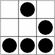
\includegraphics[height=0.5cm]{img/logo_glider.png}}

% ------------------------------------------------
% -------------   D{\'e}but document   ---------------
% ------------------------------------------------
\begin{document}
%--------- {\'e}criture de la page de titre ----------
% avec la commande frame simplifi{\'e}e
\frame[plain]{\titlepage } 
%

%------------------ Sommaire ---------------

\begin{frame}
	\frametitle{Sommaire}
	\small \tableofcontents[hideallsubsections]
\end{frame} 

\section{Cyber Fizz Buzz}
\begin{frame}
	\frametitle{Cyber Fizz Buzz}
	\tableofcontents[sections=1,currentsection,subsectionstyle=show/shaded/hide] %% sectionstyle=hide/hide,
\end{frame} 

\begin{frame}
	\frametitle{Cyber Fizz Buzz}
	
	\emph{"1, 2, Fizz, 4, Buzz, Fizz, 7, 8, Fizz, Buzz, 11, Fizz, 13, 14, Fizz Buzz, 16, 17, Fizz, 19, Buzz, Fizz, 22, 23, Fizz, Buzz, 26, Fizz, 28, 29, Fizz Buzz, 31, 32, Fizz, 34, Buzz, Fizz, ..."}~\\~\\
	
	
	Fizz buzz (often spelled FizzBuzz in this context) has been used as an interview screening device for computer programmers. Writing a program to output the first 100 FizzBuzz numbers is a relatively trivial problem requiring little more than a loop and conditional statements. However, its value in coding interviews is to analyze fundamental coding habits that may be indicative of overall coding ingenuity.

\end{frame} 

\section{Fizz Buzz K{\'e}zako ?}
\begin{frame}
	\frametitle{Fizz Buzz K{\'e}zako ?}
	\tableofcontents[sections=2,currentsection,subsectionstyle=show/shaded/hide]
\end{frame} 

\def\titleTentativeDefinitionCyberFizzBuzz{Cyber Fizz Buzz : tentative de d{\'e}finition}
\subsection{\titleTentativeDefinitionCyberFizzBuzz }
\begin{frame}
	\frametitle{\titleTentativeDefinitionCyberFizzBuzz ~(1)}
	
	"{\'E}valuation d'un candidat lors d'un entretien technique. "~\\
	
	\begin{itemize}
		\item {\'E}valuer les connaissances et r{\'e}alisations ; 
		\item {\'E}valuer les interactions (client, coll{\`e}gues, ...) ; 
		\item Conna{\^i}tre la fa\c{c}on de r{\'e}fl{\'e}chir du candidat ; 
		\item Ouverture d'esprit du candidat (critique, construction, positionnement) ; 
		\item Connaissances de technique de programmation et algorithmique ; 
	\end{itemize}~\\
	
	%% Note : Pourquoi le CyberFizzBuzz ? Formations non homog{\`e}nes (m{\^e}me au sein d'un m{\^e}me cursus). 
\end{frame}

\begin{frame}
	\frametitle{\titleTentativeDefinitionCyberFizzBuzz ~(2)}
	
	\textbf{Pourquoi le CyberFizzBuzz ?} Les formations NE sont PAS homog{\`e}nes (m{\^e}me au sein d'un m{\^e}me cursus)~\\
	
	\begin{itemize}
		\item Diff{\'e}rents cursus (ing{\'e}nieurs, universitaires, cursus cours, autodidactes), diff{\'e}rentes promotions... ;  
		\item Ressources Accessibles et Ressources Acc{\'e}d{\'e}es (Stack Overflow; 
		\item Projets r{\'e}alis{\'e}s, temps pass{\'e}, int{\'e}r{\^e}t {\`a} ce moment ; 
		\item Tutorat pendant le cursus, mentorat et encadrement par la suite ; 
		\item Exp{\'e}rience professionnelle ET personnelle !
	\end{itemize}~\\
	
	Tout ceci a un impact sur l'apprentissage par le candidat et sa restitution et tout d{\'e}pend de ce que l'on cherche {\`a} savoir !
\end{frame}

\subsection{Cyber Fizz Buzz : concepts}
\begin{frame}
	\frametitle{Cyber Fizz Buzz : concepts}
	
	\textbf{Que veut-on conna{\^i}tre et {\'e}valuer chez le candidat ?}~\\
	
	\begin{itemize}
		\item Connaissances d'un langage de programmation ; 
		\item Connaissance de concepts inh{\'e}rent {\`a} la programmation ; 
		\item {\'E}lements de culture voisine, d{\'e}finitions : 
		\begin{itemize}
			\item Divers : concepts math{\'e}matiques, optimisation, architecture de Von Neumann ; 
			\item Programmations proc{\'e}durale, fonctionnelle, orient{\'e}e objet...
			\item Gestion m{\'e}moire ; 
			\item CyberS{\'e}curit{\'e} ; 
			\item ... 
		\end{itemize}
		\item ... 
	\end{itemize}
\end{frame} 

\subsection{Cyber Fizz Buzz : int{\'e}r{\^e}ts}
\begin{frame}
	\frametitle{Cyber Fizz Buzz : int{\'e}r{\^e}ts}
	
	\textbf{L'objectif est-il seulement d'{\'e}valuer les comp{\'e}tences technique ?} NON !~\\
	\emph{Analyse de la d{\'e}marche de r{\'e}solution de probl{\`e}mes. }
	
	\begin{itemize}
		\item Capacit{\'e} {\`a} formuler "Je ne sais pas. " (et comment savoir) ; 
		\item Capacit{\'e} {\`a} {\'e}changer / dialoguer (pendant l'entretien) ; 
		\item M{\'e}thodologies utilis{\'e}es (Tests Unitaires, It{\'e}rations, Objets, {\'E}num{\'e}rations, Fonctions, Patrons de Conception...)
		\item D{\'e}marche de documentation, de veille, de recherche d'information ; 
		\item Publication de projets, en partie ou en totalit{\'e} ; 
		\item ... 
	\end{itemize}
\end{frame} 

\def\titleExemplesCyberFizzBuzz{CyberFizzBuzz : Concepts et Exemples}
\section{\titleExemplesCyberFizzBuzz }
\begin{frame}
	\frametitle{\titleExemplesCyberFizzBuzz }
	\tableofcontents[sections=3,currentsection,subsectionstyle=show/shaded/hide]
\end{frame} 

\subsection{\titleExemplesCyberFizzBuzz ~(1)}
\begin{frame}
	\frametitle{C\titleExemplesCyberFizzBuzz ~(1)}
	\begin{itemize}
		\item {\`A} partir d'un {\'e}nonc{\'e} de base, construction tests et codes avec commentaires et explications ; 
		\item L'objectif principal n'est pas de r{\'e}aliser l'ensemble du projet d{\'e}crit dans l'{\'e}nonc{\'e} ; 
		\item Exercice volontairement trop long pour le temps imparti ; 
		\item Analyse du cheminement (architecture et approche utilis{\'e}es par le candidat), plut{\^o}t que le r{\'e}sultat ;
		\item Questions compl{\'e}mentaires {\`a} partir de l'{\'e}nonc{\'e} (interaction) ; 
	\end{itemize}
\end{frame} 

\subsection{\titleExemplesCyberFizzBuzz ~(2)}
\begin{frame}
	\frametitle{\titleExemplesCyberFizzBuzz ~(2)}
	\begin{itemize}
		\item Impl{\'e}mentations de structures / classes, tests unitaires... ;
		\item Optimisations, Approches utilis{\'e}es (TDD, DDD...) ; ... 
		\item {\'E}crire une suite de nombres (for, stream, lambdas)...
		\item Op{\'e}rateur modulo (\%) : peu utilis{\'e} mais alternatives ; 
		\item Interfaces et Classes, Design Patterns (concepts et applications) ; 
		\item Abstractions et Interfaces de POO ; 
		\item D{\'e}marche TDD, Utilisation de Git, Cr{\'e}ation de microservices (REST)...
	\end{itemize}
\end{frame} 

\subsection{\titleExemplesCyberFizzBuzz ~(3)}
\begin{frame}
	\frametitle{\titleExemplesCyberFizzBuzz ~(3)}
	\begin{itemize}
		\item Analyser logique d'un algorithme : entier ou r{\'e}el le plus proche d'une valeur donn{\'e}e ; 
		\item Recherche dans une matrice ; 
		\item Parcours d'arbres (classification, valeurs, tri...) ; 
		\item[] 
		\item Un {\'e}nonc{\'e} volontairement vaste, non-r{\'e}alisable dans le temps de l'entretien (1 heure {\`a} 1 heure 30) et qui peut {\^e}tre compl{\'e}t{\'e} dans un temps raisonnable en-dehors (pas plus de 3-5 heures) ; 
		\item Non-n{\'e}cessaire en interne (ce n'est pas l'objectif, ni d'externaliser, ni de donner un exemple) ; 
	\end{itemize}
\end{frame} 

\subsection{\titleExemplesCyberFizzBuzz ~(4)}
\begin{frame}
	\frametitle{\titleExemplesCyberFizzBuzz ~(4)}
	\begin{itemize}
		\item $\rightarrow$ Un monnayeur (machine {\`a} rendre la monnaie),~\newline \emph{"Slot Machine"} ;
		\item $\rightarrow$ Jeu de cartes de combats 'Monstres et Sortil{\`e}ges',~\newline{"RPG Cards"} ;
		\item $\rightarrow$ Un syst{\`e}me de commandes {\'e}volutif sans changement de structure de contr{\^o}le (Strategy / Command : utiliser autre chose que Switch et IF) ;
		\item $\rightarrow$ Un jeu de morpion quantique avec Web-Services,~\newline{"Quantum Tic-Tac-Toe With REST"} ; idem FizzBuzz en REST ;
		\item $\rightarrow$ Un projet simple avec it{\'e}rations : "Coffee Machine Project" ; 
		\item $\rightarrow$ ...
	\end{itemize}
\end{frame} 

\subsection{\titleExemplesCyberFizzBuzz ~(5)}
\begin{frame}
	\frametitle{\titleExemplesCyberFizzBuzz ~(5)}
	\begin{itemize}
		\item Optimisation : r{\'e}cursivit{\'e}, it{\'e}rativit{\'e}, m{\'e}moire tampon... \emph{Fibonacci}
		\item Exhaustivit{\'e} : tests {\`a} vide, tests {\`a} \emph{null}, grandes valeurs / grands ensembles...
		\item Expressivit{\'e} : expliquer, documenter, terminologie explicit{\'e}e... 
		\item ...
		\item Ce n'est pas forc{\'e}ment {\`a} v{\'e}rifier strictement aupr{\`e}s du candidat, plus dans l'objectif d'un {\'e}tat d'esprit.
		\item ... 
		\item Que faire si refus de r{\'e}aliser un test technique ? Possible !
	\end{itemize}
\end{frame} 

\section{Qu'est-ce que l'on fait de tout \c{c}a ?}
\begin{frame}
	\frametitle{Qu'est-ce que l'on fait de tout \c{c}a ?}
	\tableofcontents[sections=4,currentsection,subsectionstyle=show/shaded/hide] %% sectionstyle=hide/hide,
\end{frame} 

\subsection{Poser les {\'e}l{\'e}ments dont on a besoin. }
\begin{frame}
	\frametitle{Poser les {\'e}l{\'e}ments dont on a besoin. }
	\begin{itemize}
		\item Comp{\'e}tences techniques, conceptuelles ; 
		\item Comp{\'e}tences n{\'e}cessaires ; 
		\item Comp{\'e}tences optionnelles (int{\'e}ressantes {\`a} avoir) ; 
		\item Comp{\'e}tences optionnelles (mont{\'e}e en comp{\'e}tence possible) ;
		\item Comp{\'e}tences non-techniques (relationnelles / "soft-skills") ;  
		\item ... 
	\end{itemize}
\end{frame} 

\subsection{Comment {\'e}value-t-on ?}
\begin{frame}
	\frametitle{Comment {\'e}value-t-on ?}
	\begin{itemize}
		\item Qualifiable (purement bool{\'e}en : absent / pr{\'e}sent ; ou granularit{\'e} : niveau voulu) ; 
		\item Quantifiable (nombre de r{\'e}ponses ou d'{\'e}l{\'e}ments pr{\'e}sent) ; 
		\item "Questions {\'e}liminatoires" ({\'e}l{\'e}ments non pr{\'e}sents, ou r{\'e}dhibitoires) ; 
		\item Part de subjectivit{\'e} et autres marges de man\oe uvre ; 
		\item ... 
	\end{itemize}~\\
	
	Ne pas oublier le contexte d'{\'e}valuation : pendant l'entretien ? Test technique {\`a} part ?
\end{frame}

\subsection{Faire {\'e}voluer son test de recrutement}
\begin{frame}
	\frametitle{Faire {\'e}voluer son test de recrutement}
	\begin{itemize}
		\item Retours des candidats sur le recrutement ; 
		\item Niveaux de difficult{\'e}s (questions, r{\'e}ponses attendues, d{\'e}marches...) ; 
		\item Diff{\'e}rents tests (profils, langages de programmation, postes...) ; 
		\item Renouvellement (changement de version de ce qui est test{\'e}, et {\'e}viter le "bachotage") ; 
		\item ... 
	\end{itemize}~\\
	
\end{frame} 

\subsection{D'autres ressources (1)}
\begin{frame}
	\frametitle{D'autres ressources (1)}
	\begin{itemize}
		\small
		\item ``An incomplete list of skills senior engineers need, beyond coding''~\\
			\texttt{\footnotesize https://skamille.medium.com/an-incomplete-list-of-skills-senior-engineers-need-beyond-coding-8ed4a521b29f }
		\item ``Love Them or Hate Them, Coding Exercises Are an Essential Part of Software Engineering Interviews ''~\\
			\texttt{\footnotesize https://dev.to/thawkin3/love-them-or-hate-them-coding-exercises-are-an-essential-part-of-software-engineering-interviews-3odd }
		\item You are Not Google / Amazon / ... (Nobody is !)~\\
			\texttt{\footnotesize https://blog.bradfieldcs.com/you-are-not-google-84912cf44afb }
		\item Software Engineering Links : \texttt{\footnotesize https://gist.github.com/vineus/06c9760cbe922e97d549962768ad0146 }
		\item ... 
	\end{itemize}~\\
	
\end{frame} 

\subsection{D'autres ressources (2)}
\begin{frame}
	\frametitle{D'autres ressources (2)}
	\begin{itemize}
		\item \emph{Geek / Nerd / Pop Culture ? (Not Only Programmers And What You Can See From Them !)}
		\item Probablement d'autres passions que le code informatique et les outils associ{\'e}s (et pas forc{\'e}ment non plus des clich{\'e}s limitatifs autours des jeux vid{\'e}o, des mangas et du rock m{\'e}tal...) ;
		\item Tests Techniques : et d'autres mises en situation ? ; 
		\item Aspects relationnel : comment tester en restant objectif ?
		\item Travail en {\'e}quipe : au-del{\`a} d'un syst{\`e}me comp{\'e}titif ;  
		\item ... 
	\end{itemize}~\\
	
\end{frame} 

\def\sectionPartBibliographie{Bibliographie / Mediagraphie}
\section{\sectionPartBibliographie}
\begin{frame}
	\frametitle{\sectionPartBibliographie}
	\nocite{*}
	%toutes references biblio : 6 lettres + 2 chiffres
	\bibliography{presentationCyberFizzBuzz}
	% \bibliographystyle{frplain} % plain or frplain
	\bibliographystyle{plain}
\end{frame}

\end{document}
